\documentclass[12pt,a4paper]{article}

%--------------------------------
% PAQUETES
%--------------------------------
\usepackage[spanish]{babel}
\usepackage[utf8]{inputenc}
\usepackage[T1]{fontenc}
\usepackage{geometry}
\usepackage{graphicx}
\usepackage{float}
\usepackage{amsmath}
\usepackage{booktabs}
\usepackage{multirow}
\usepackage{enumitem}
\usepackage[colorlinks=true, linkcolor=blue, urlcolor=blue]{hyperref}

\geometry{margin=2.5cm}

% Marcas de plantilla: se dejan como contenido directo para que el documento compile.

%--------------------------------
% DATOS DEL INFORME (COMPLETAR)
%--------------------------------

%--------------------------------
\begin{document}

%--------------------------------
% PORTADA
%--------------------------------
\begin{titlepage}
    \centering

    {\scshape\LARGE Universidad Tecnológica Nacional \par}
    \vspace{0.3cm}
    {\scshape\Large Facultad Regional Córdoba \par}
    \vspace{1.5cm}

    {\scshape\Large Dispositivos Electrónicos I \par}
    \vspace{2cm}

    {\Huge\bfseries Trabajo Práctico N°1 \par}
    \vspace{0.5cm}
    {\LARGE Identificación de Componentes Electrónicos y
Mediciones Básicas \par}

    \vspace{2cm}

    \begin{flushleft}
    \textbf{Integrantes:} \\
    Alejos Antony --- 412820 --- Operador\\
    Cortesini Luciano --- 402719 --- Coordinador\\
    Pedregoza Juan --- 408644 --- Documentador\\

    \vspace{0.5cm}

    \textbf{Curso:} 3R3 \\
    \textbf{Grupo:} 02 \\
    \textbf{Docente:}  Leonardo Gabriel Gamboa\\
    \textbf{Año:} 2026 \\
    \end{flushleft}

    \vfill

\end{titlepage}
\thispagestyle{empty}

\vspace{1cm}

\tableofcontents
\newpage

 
% ══════════════════════════════════════════════════════════════════════════════
\section{Análisis del Circuito}
 
El circuito analizado corresponde a la figura 5 de la guía, con los siguientes
parámetros de diseño:
 
\begin{itemize}
    \item $V_S = 10\,\text{V}$
    \item $R_1 = 10\,\text{k}\Omega$
    \item $R_2 = 4{,}7\,\text{k}\Omega$
    \item $R_3 = 3{,}3\,\text{k}\Omega$
\end{itemize}
 
El circuito consiste en $R_1$ en serie con la fuente $V_S$, mientras que $R_2$
y $R_3$ se encuentran en paralelo entre sí y en serie con $R_1$.
 
\subsection{Desarrollo teórico}
 
A continuación se plantean las ecuaciones y se resuelven los valores de tensión,
corriente y potencia para cada elemento.
 
\subsubsection{Resistencia equivalente del paralelo $R_2 \| R_3$}
 
\begin{equation}
    R_{23} = \frac{R_2 \cdot R_3}{R_2 + R_3}
    = \frac{4{,}7\,\text{k}\Omega \cdot 3{,}3\,\text{k}\Omega}
           {4{,}7\,\text{k}\Omega + 3{,}3\,\text{k}\Omega}
    = {1{,}94}\,\text{k}\Omega
\end{equation}
 
\subsubsection{Resistencia total del circuito}
 
\begin{equation}
    R_T = R_1 + R_{23}
    = 10\,\text{k}\Omega + {1{,}94}\,\text{k}\Omega
    = {11{,}94}\,\text{k}\Omega
\end{equation}
 
\subsubsection{Corriente total entregada por la fuente}
 
Por Ley de Ohm:
 
\begin{equation}
    I_T = \frac{V_S}{R_T}
    = \frac{10\,\text{V}}{{11{,}94}\,\text{k}\Omega}
    = {837{,}6}\,\mu\text{A}
\end{equation}
 
\subsubsection{Tensiones en cada elemento}
 
Aplicando la Ley de Tensiones de Kirchhoff (LVK) en la malla principal:
 
\begin{align}
    V_{R1} &= I_T \cdot R_1 = {837{,}6}\,\mu\text{A} \cdot 10\,\text{k}\Omega = {8{,}376}\,\text{V} \\
    V_{R2} &= V_{R3} = V_S - V_{R1} = 10\,\text{V} - {8{,}37}\,\text{V} = {1{,}624}\,\text{V}
\end{align}
 
\subsubsection{Corrientes en $R_2$ y $R_3$}
 
Aplicando la Ley de las Corrientes de Kirchhoff (LKI) en el nodo B:
 
\begin{align}
    I_2 &= \frac{V_{R2}}{R_2} = \frac{1{,}624\,\text{V}}{4{,}7\,\text{k}\Omega} = 345{,}5\,\mu\text{A} \\
    I_3 &= \frac{V_{R3}}{R_3} = \frac{1{,}624\,\text{V}}{3{,}3\,\text{k}\Omega} = 492{,}1\,\mu\text{A}
\end{align}
 
Verificación LKI: $I_T = I_2 + I_3 = X{,}XX\,\text{mA}$ (verificado)
 
\subsubsection{Potencias}
 
\begin{align}
    P_{VS}  &= V_S \cdot I_T                    = 8{,}376\,\text{mW} \\
    P_{R1}  &= I_T^2 \cdot R_1                  = 7{,}016\,\text{mW} \\
    P_{R2}  &= \frac{V_{R2}^2}{R_2}             = 0{,}561\,\text{mW} \\
    P_{R3}  &= \frac{V_{R3}^2}{R_3}             = 0{,}799\,\text{mW}
\end{align}
 
Balance de potencias: $P_{VS} = P_{R1} + P_{R2} + P_{R3}$ (verificado)
 
\subsection{Tabla de valores calculados}
 
\begin{table}[H]
\centering
\caption{Tabla 1 --- Valores calculados (análisis teórico)}
\renewcommand{\arraystretch}{1.5}
\begin{tabular}{lcccc}
\toprule
 & $V_S$ & $R_1$ & $R_2$ & $R_3$ \\
\midrule
Tensión   & 10V & 8,376V & 1,623V & 1,623V \\
Corriente   &  $837{,}6\,\mu\text{A}$ & $837{,}6\,\mu\text{A}$ & $345{,}5\,\mu\text{A}$ & $492{,}1\,\mu\text{A}$ \\
Potencia    &  $8{,}376\,\text{mW}$ & $7{,}016\,\text{mW}$  & $0{,}561\,\text{mW}$ & $0{,}799\,\text{mW}$ \\
\bottomrule
\end{tabular}
\end{table}
 
% ══════════════════════════════════════════════════════════════════════════════
\section{Simulación en LTspice}
 
\subsection{Simulación DC Operating Point}
 
\subsubsection{Esquemático del circuito}
 
\begin{figure}[H]
    \centering
    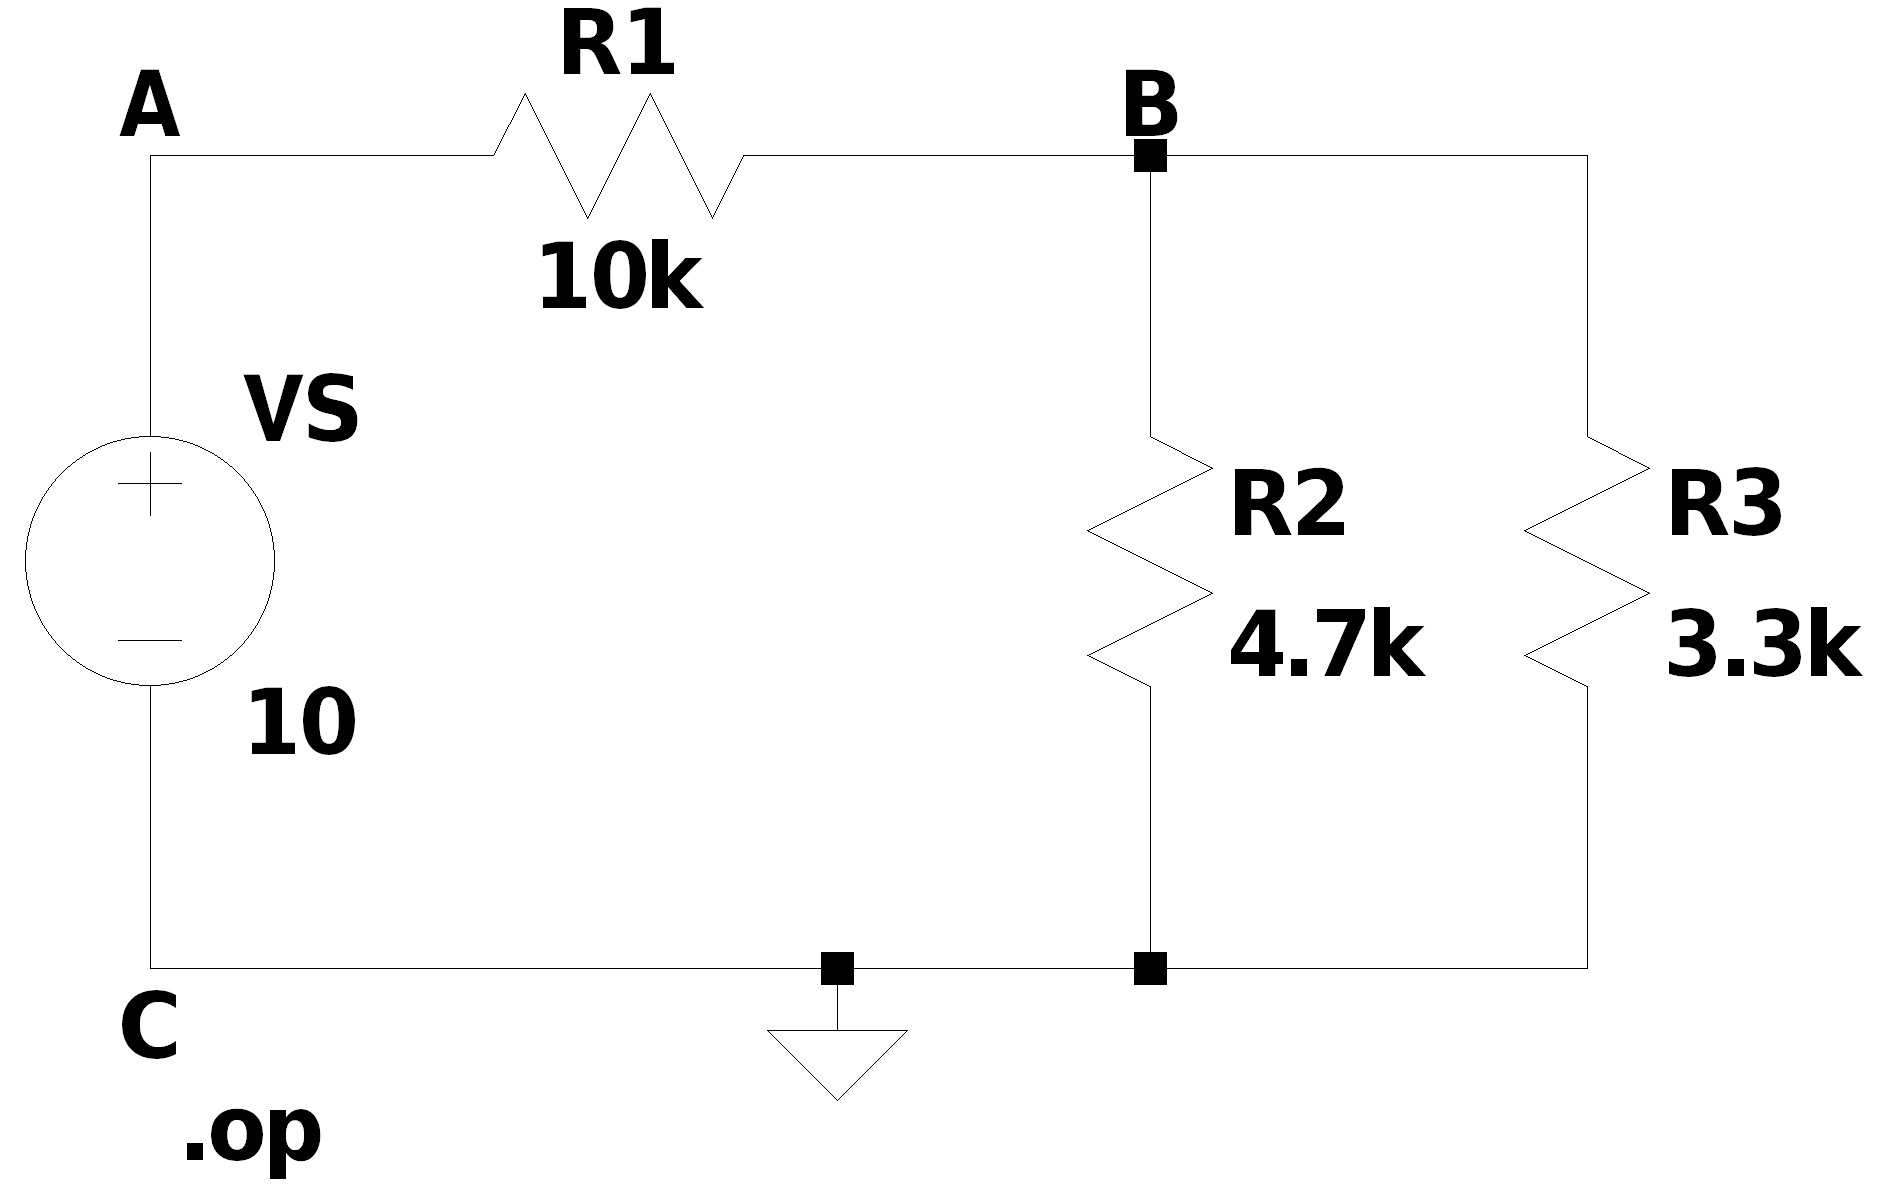
\includegraphics[width=0.60\textwidth]{image/ltspice_esquematico.png}
    \caption{Circuito esquemático armado en LTspice.}
\end{figure}
 
\subsubsection{Resultados de la simulación DC op point}
 
\begin{figure}[H]
    \centering
    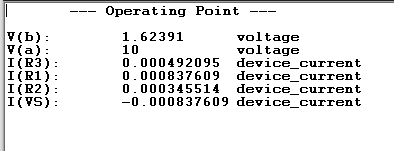
\includegraphics[width=0.70\textwidth]{image/ltspice_resultado_op.png}
    \caption{Ventana de resultados de simulación DC op point.}
\end{figure}
 
\subsubsection{Tabla de valores simulados}
 
\begin{table}[H]
\centering
\caption{Tabla 2 --- Valores obtenidos por simulación DC op point}
\renewcommand{\arraystretch}{1.5}
\begin{tabular}{lcccc}
\toprule
Elemento & Tensión (V) & Corriente (mA) & Potencia (mW) \\
\midrule
$V_S$ & $10$ & $0{,}838$ & $8{,}376$ \\
$R_1$ & $8{,}376$ & $0{,}838$ & $7{,}016$ \\
$R_2$ & $1{,}624$ & $0{,}346$ & $0{,}561$ \\
$R_3$ & $1{,}624$ & $0{,}492$ & $0{,}799$ \\
\bottomrule
\end{tabular}
\end{table}
 
Respecto al signo negativo de la potencia entregada por $V_S$ en LTspice:
[Explicar brevemente a qué se debe el signo negativo en la potencia de la fuente.]
 
Balance de potencias verificado: $P_{VS} = P_{R1} + P_{R2} + P_{R3}$:
{[Indicar si se verifica o no, y los valores correspondientes.]}
 
\subsection{Barrido de Tensión Continua (DC Sweep)}
 
\subsubsection{Configuración utilizada}
 
Comando de simulación: \texttt{.dc VS 0 20 0.1}
 
\begin{figure}[H]
    \centering
    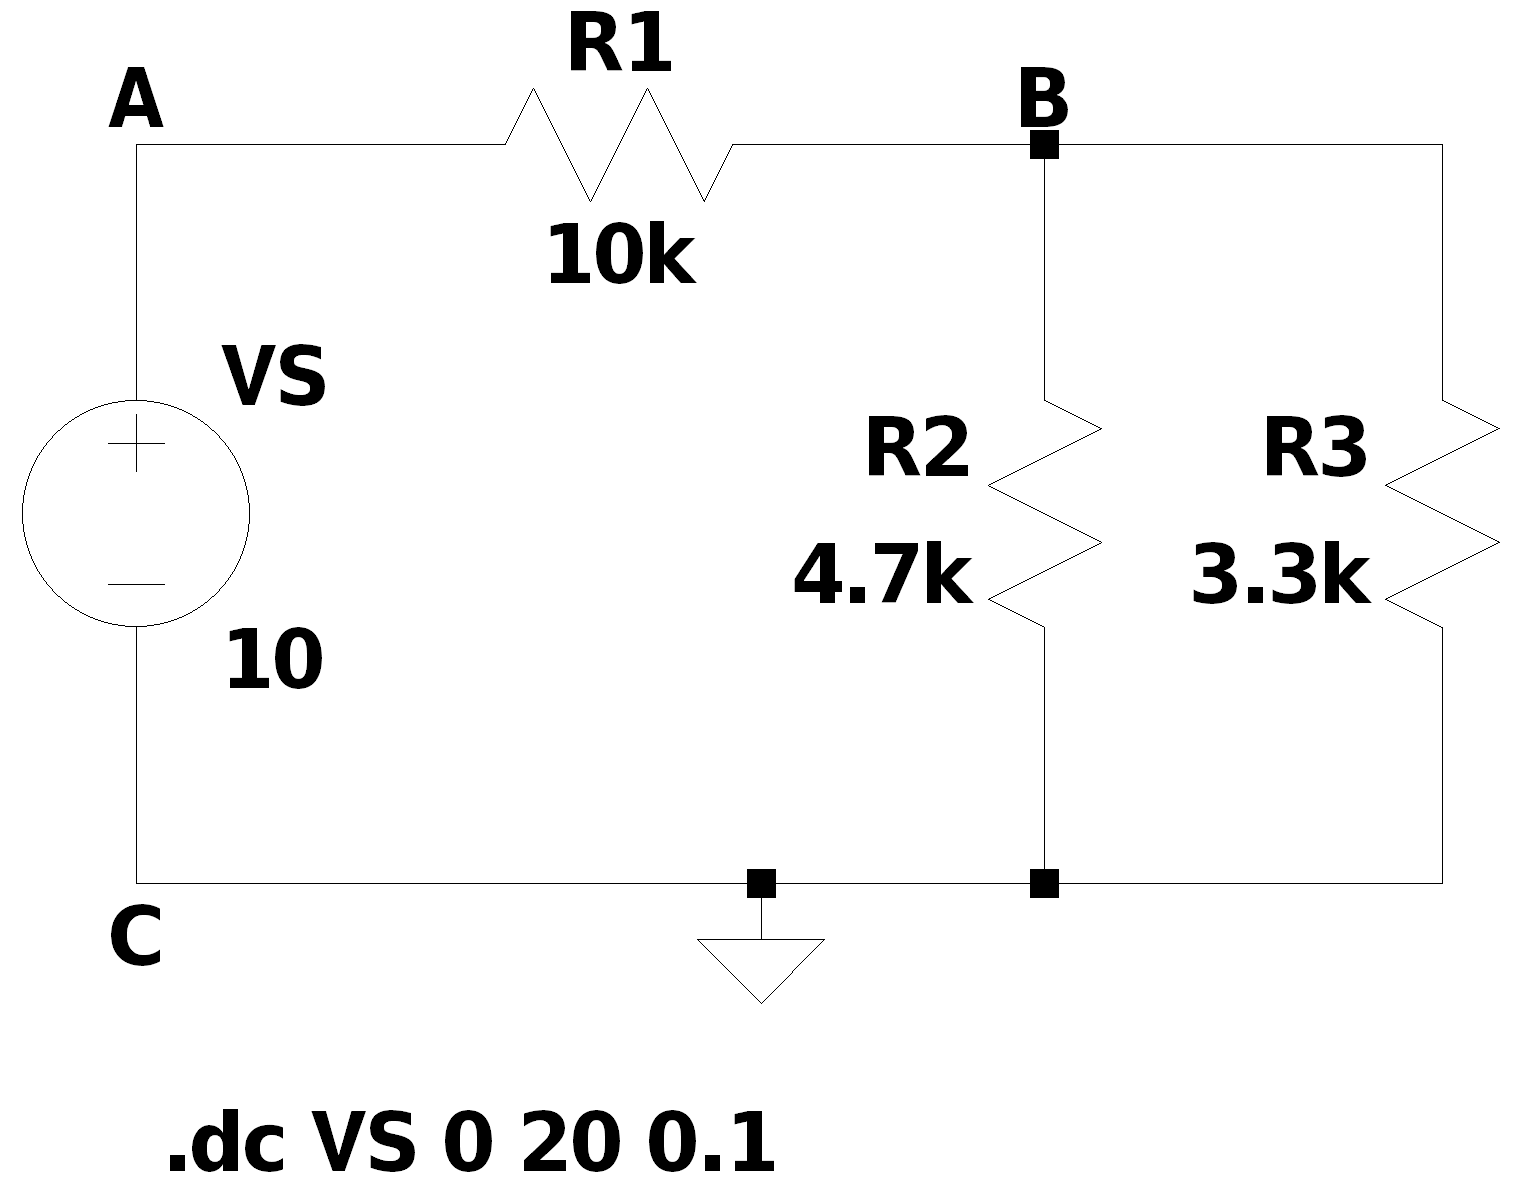
\includegraphics[width=0.60\textwidth]{image/ltspice_dcsweep_esquema.png}
    \caption{Esquemático en LTspice con directiva de DC Sweep.}
\end{figure}
 
\subsubsection{Curvas $V = f(I)$ para $R_1$, $R_2$ y $R_3$}
 
\begin{figure}[H]
    \centering
    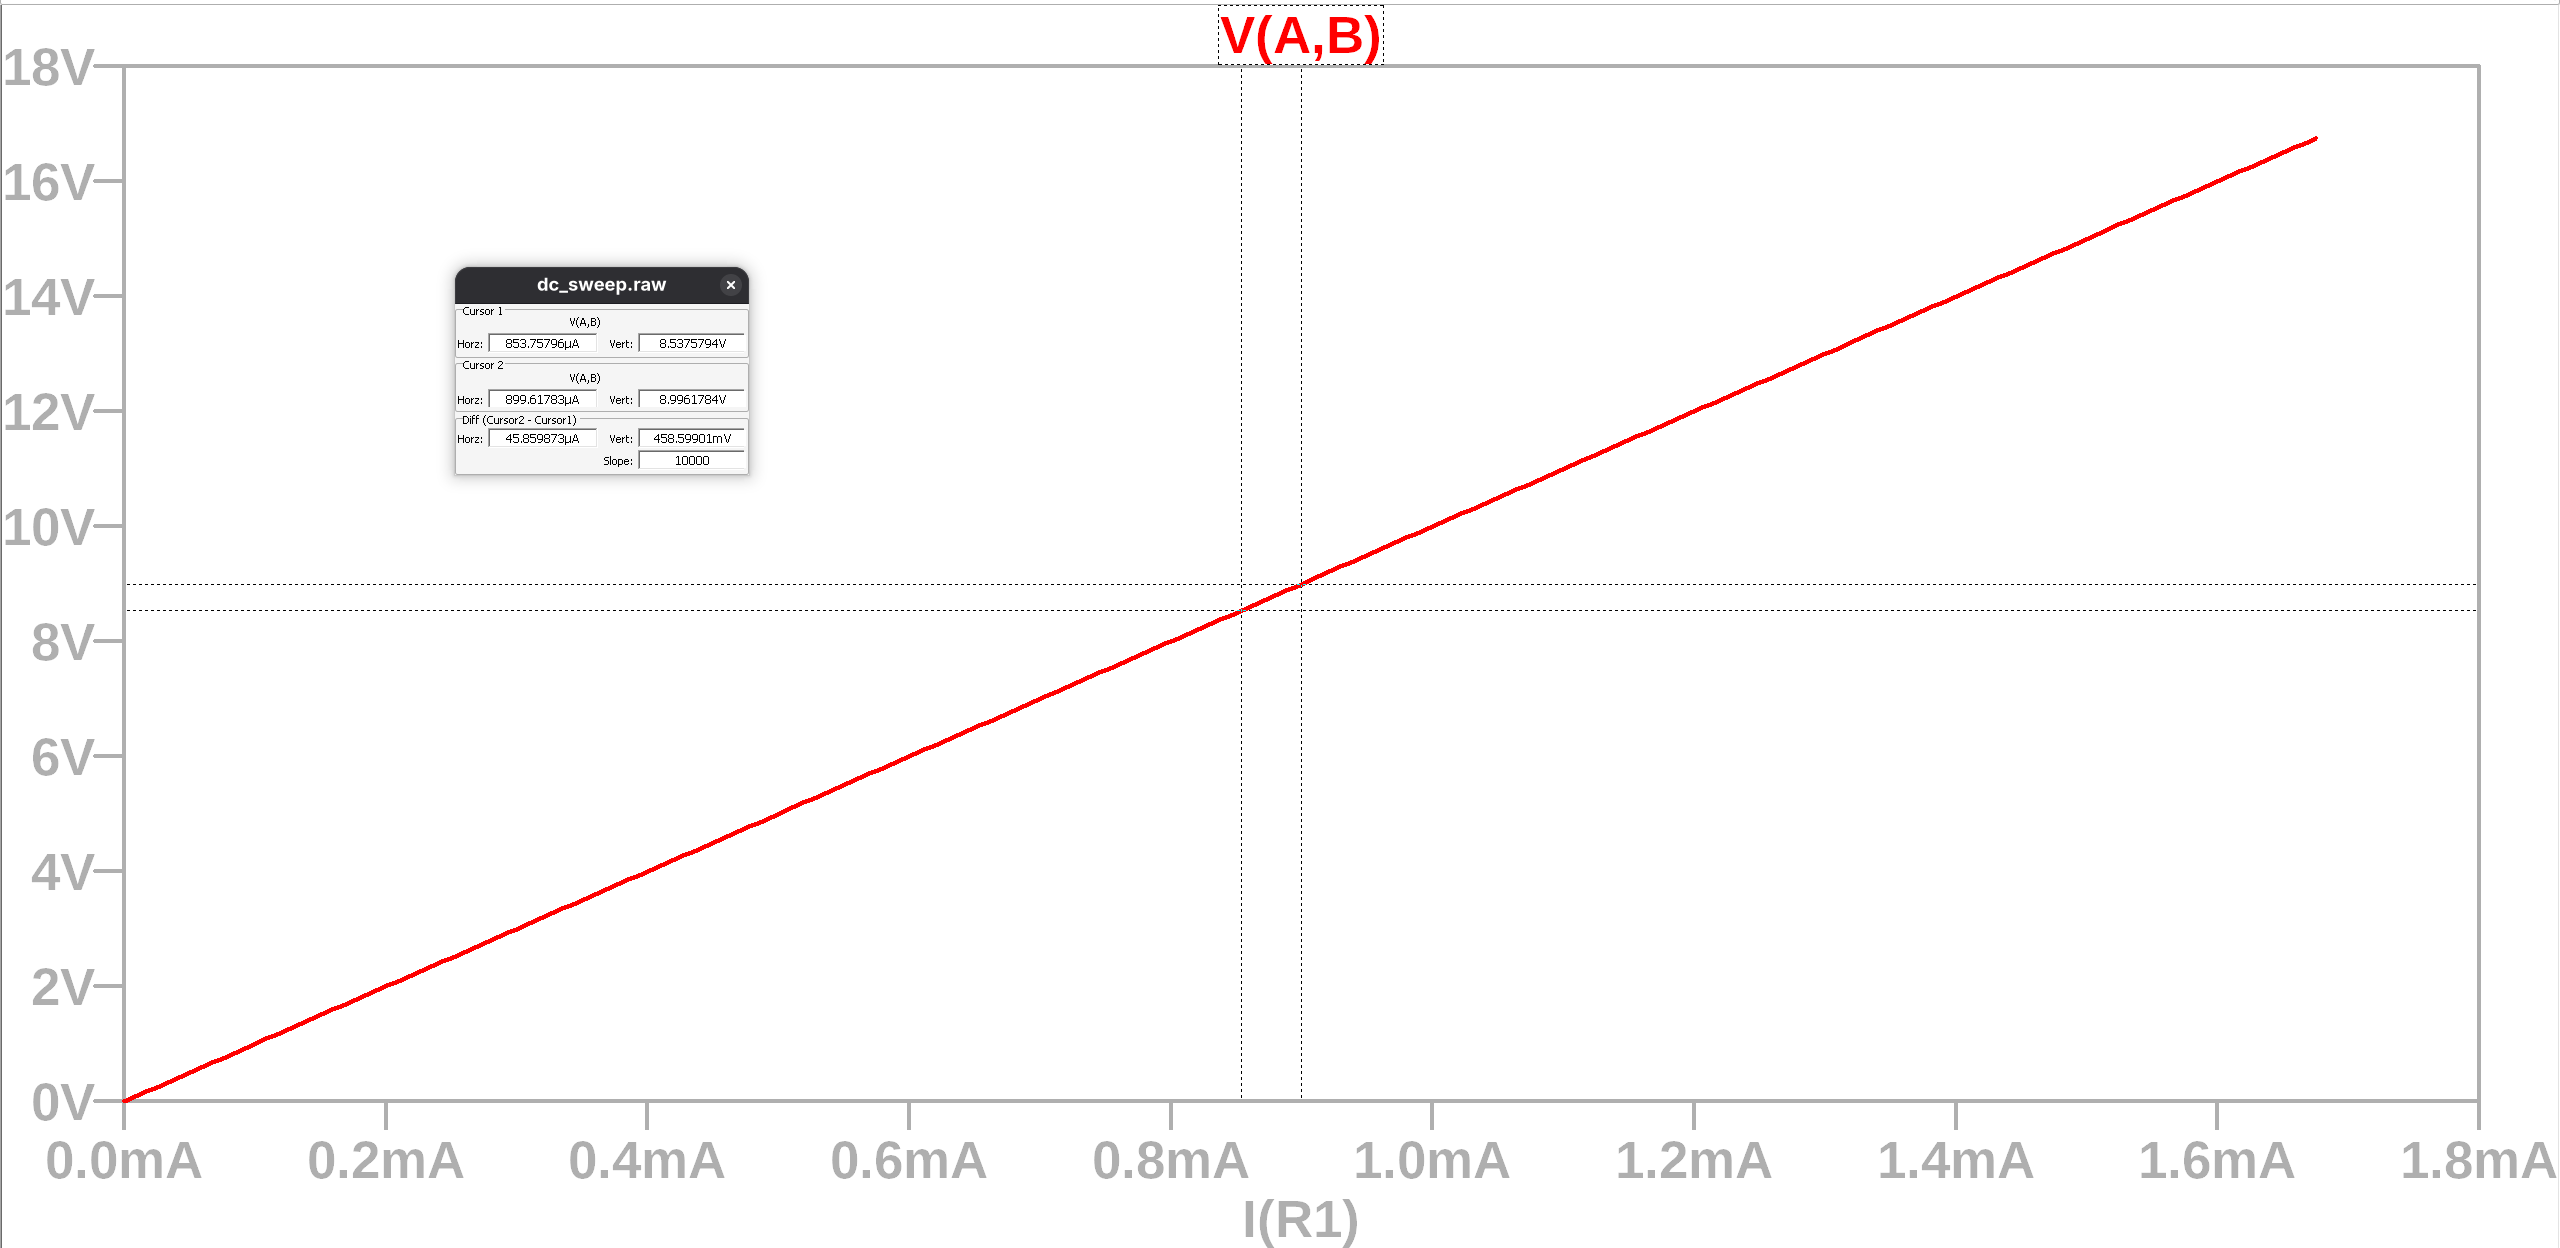
\includegraphics[width=1\textwidth]{image/ltspice_dcsweep_1.png}
    \caption{Curva de tensión vs corriente en $R_1$.}\label{fig:dcsweep_r1}
\end{figure}
\begin{figure}[H]
    \centering
    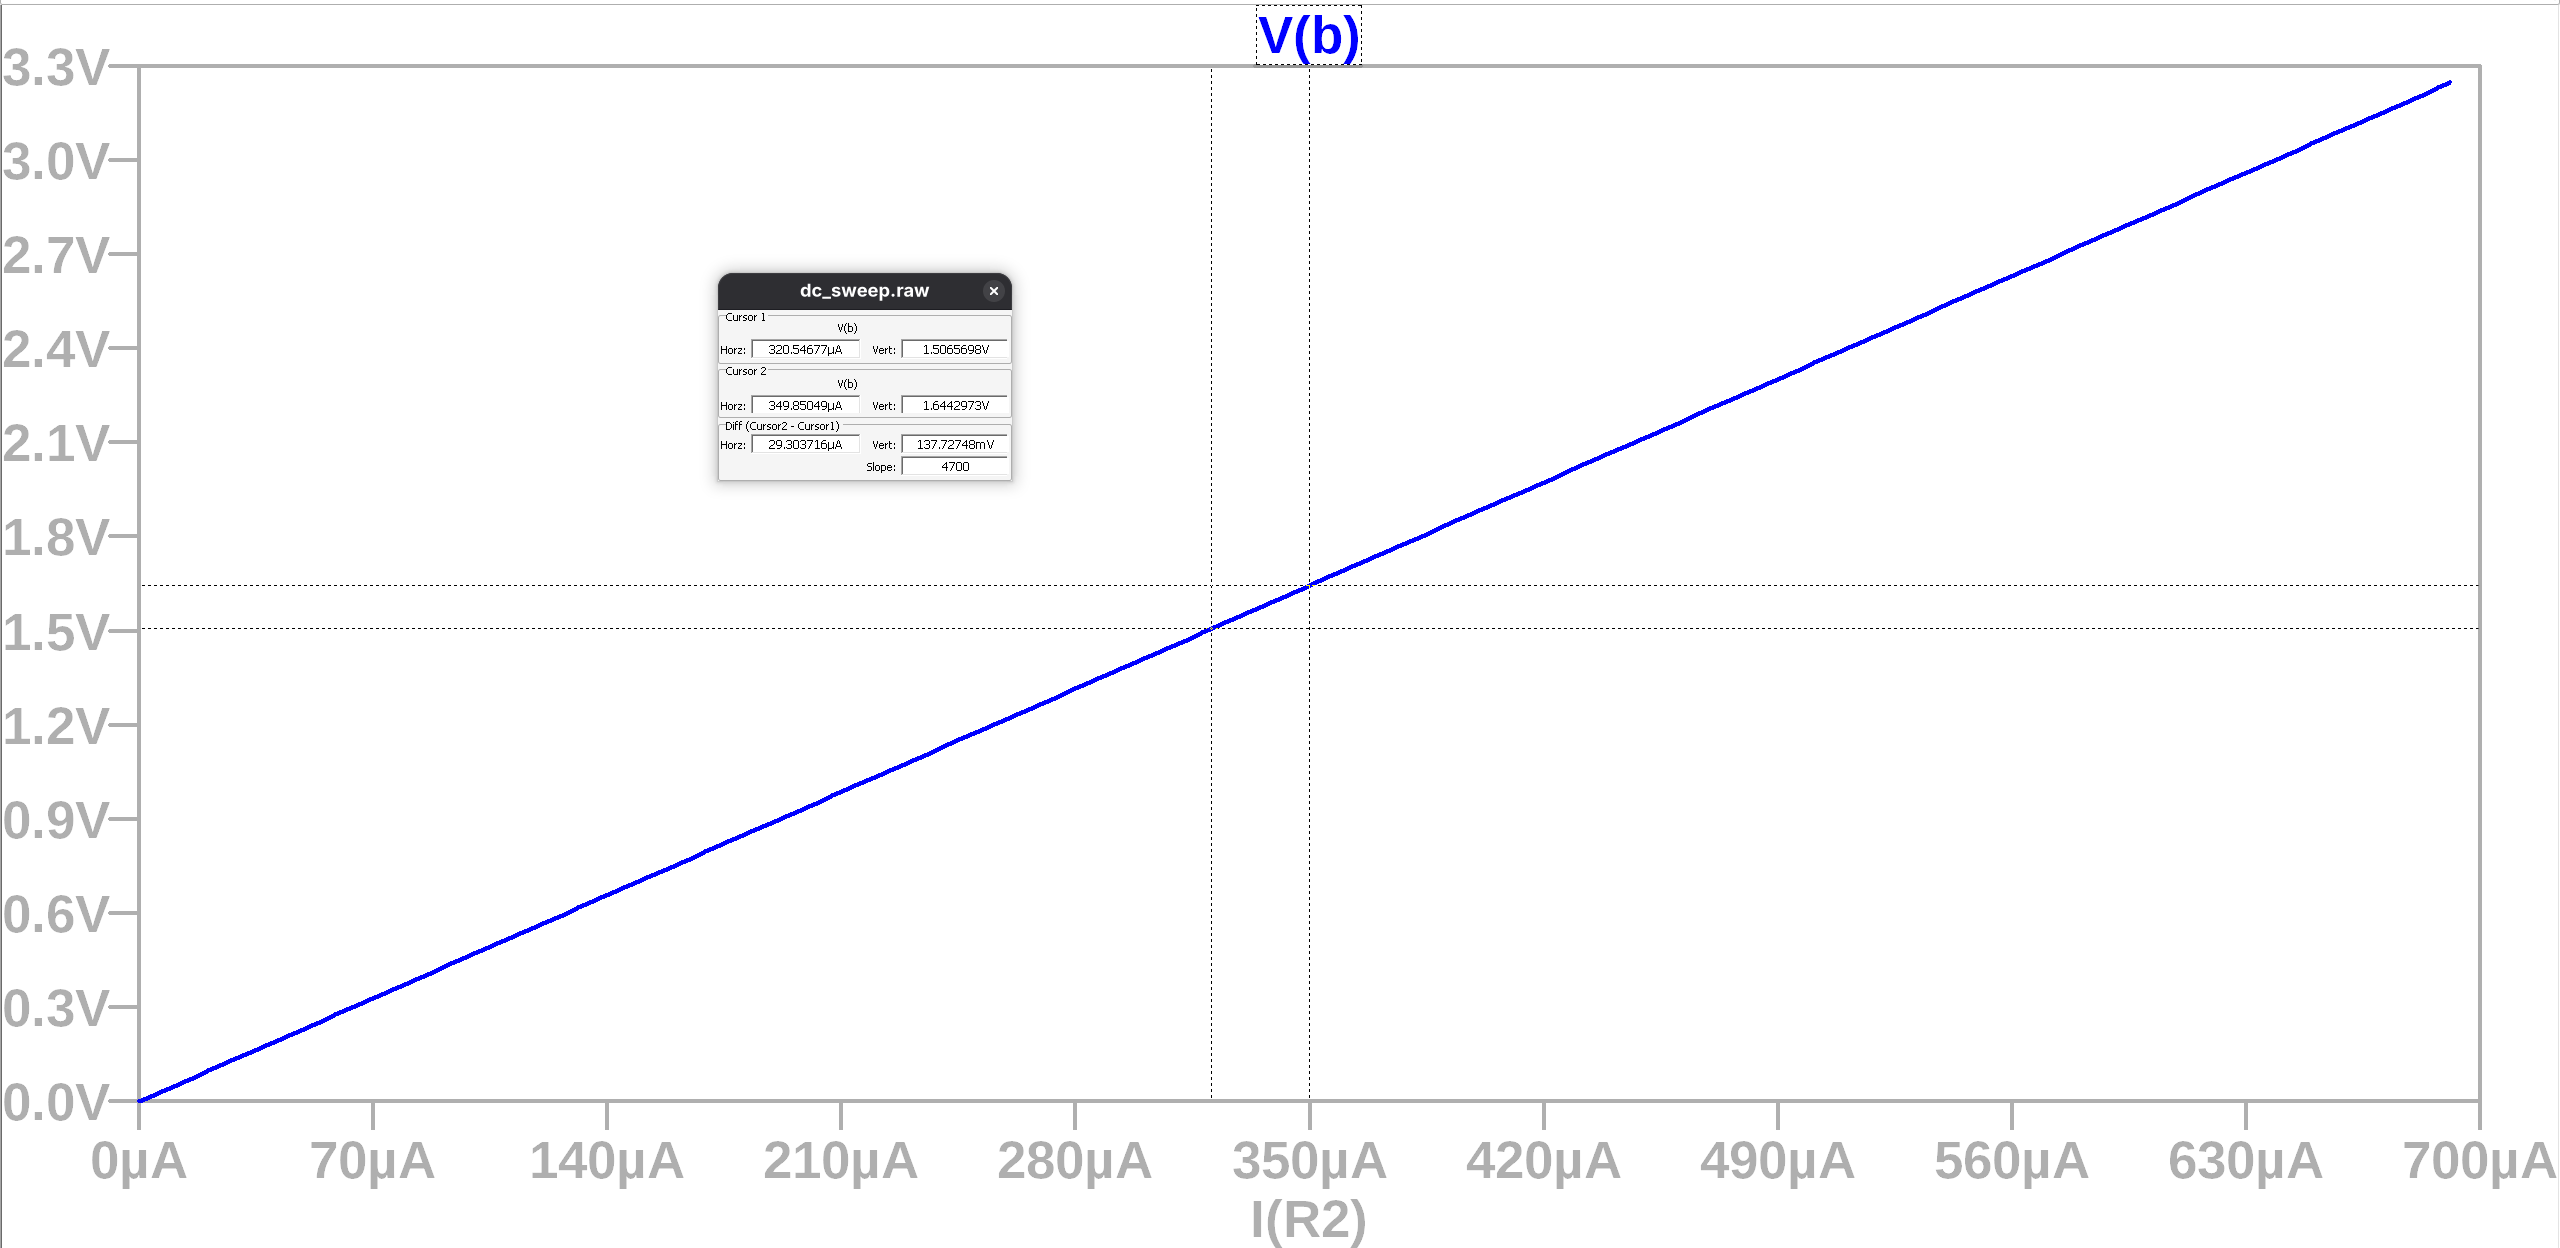
\includegraphics[width=1\textwidth]{image/ltspice_dcsweep_2.png}
    \caption{Curva de tensión vs corriente en $R_2$.}\label{fig:dcsweep_r2}
\end{figure}
\begin{figure}[H]
    \centering
    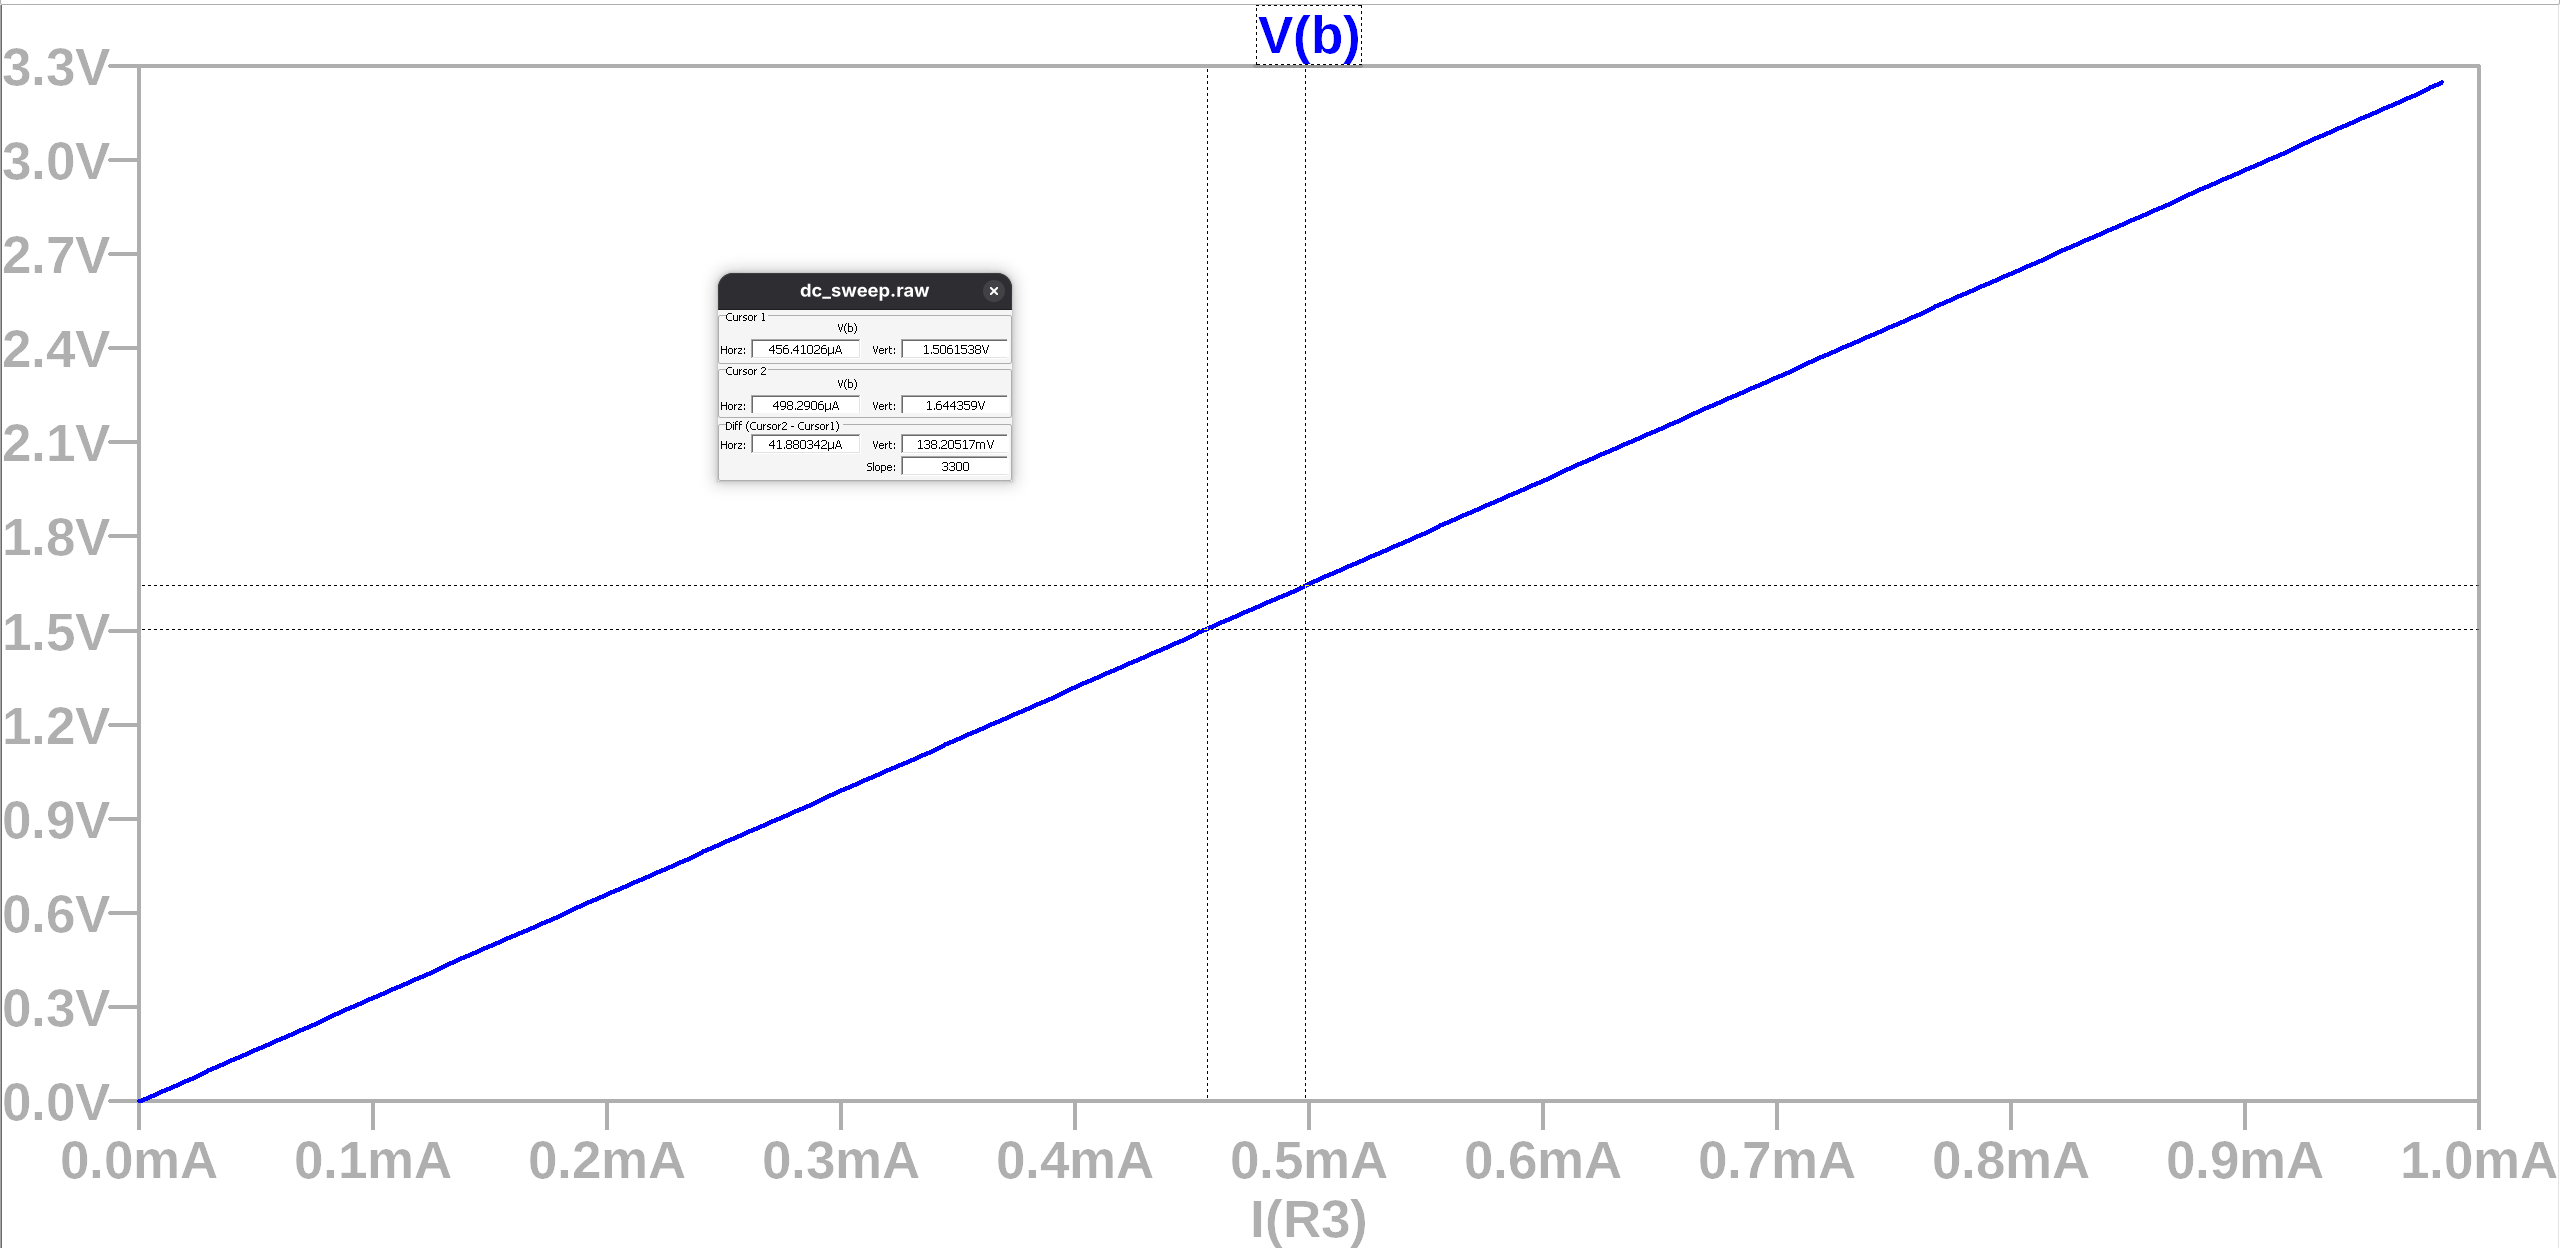
\includegraphics[width=1\textwidth]{image/ltspice_dcsweep_3.png}
    \caption{Curva de tensión vs corriente en $R_3$.}\label{fig:dcsweep_r3}
\end{figure}

En las Figuras~\ref{fig:dcsweep_r1},~\ref{fig:dcsweep_r2} y~\ref{fig:dcsweep_r3} se observan las curvas características
de cada resistencia, mostrando la relación lineal entre tensión y corriente, consistente con la Ley de Ohm. La pendiente
de cada curva corresponde al valor de la resistencia, pudimos comprobar esto utilizando dos cursores en LTSpice, que nos
devuelve la pendiente en el tramo entre ambos puntos.

\subsection{Barrido de Parámetros (Parameter Sweep)}
 
\subsubsection{Configuración utilizada}
 
Directiva SPICE utilizada: \texttt{.step param Rval 1k 10k 1k}

$R_2$ fue reemplazada por el parámetro \texttt{\{Rval\}}, variando desde
$1\,\text{k}\Omega$ hasta $10\,\text{k}\Omega$ en pasos de $1\,\text{k}\Omega$.
 
\begin{figure}[H]
    \centering
    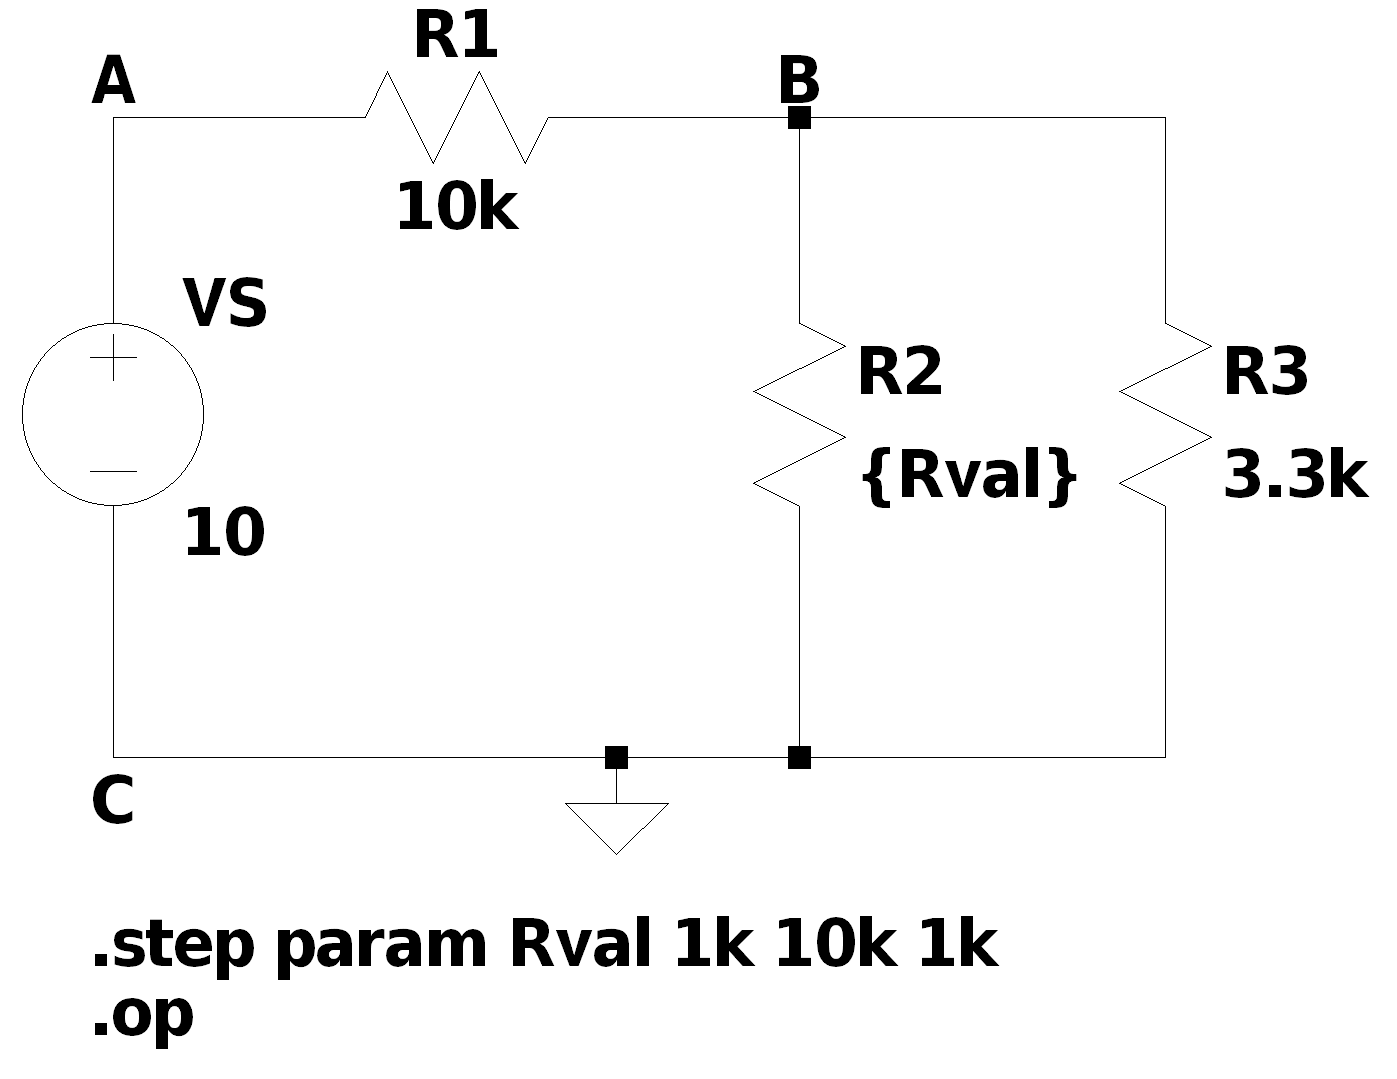
\includegraphics[width=0.60\textwidth]{image/ltspice_paramsweep_esquema.png}
    \caption{Esquemático con parámetro \texttt{\{Rval\}} en $R_2$.}
\end{figure}
 
\subsubsection{Gráficas de tensión y corriente en nodo B}
 
\begin{figure}[H]
    \centering
    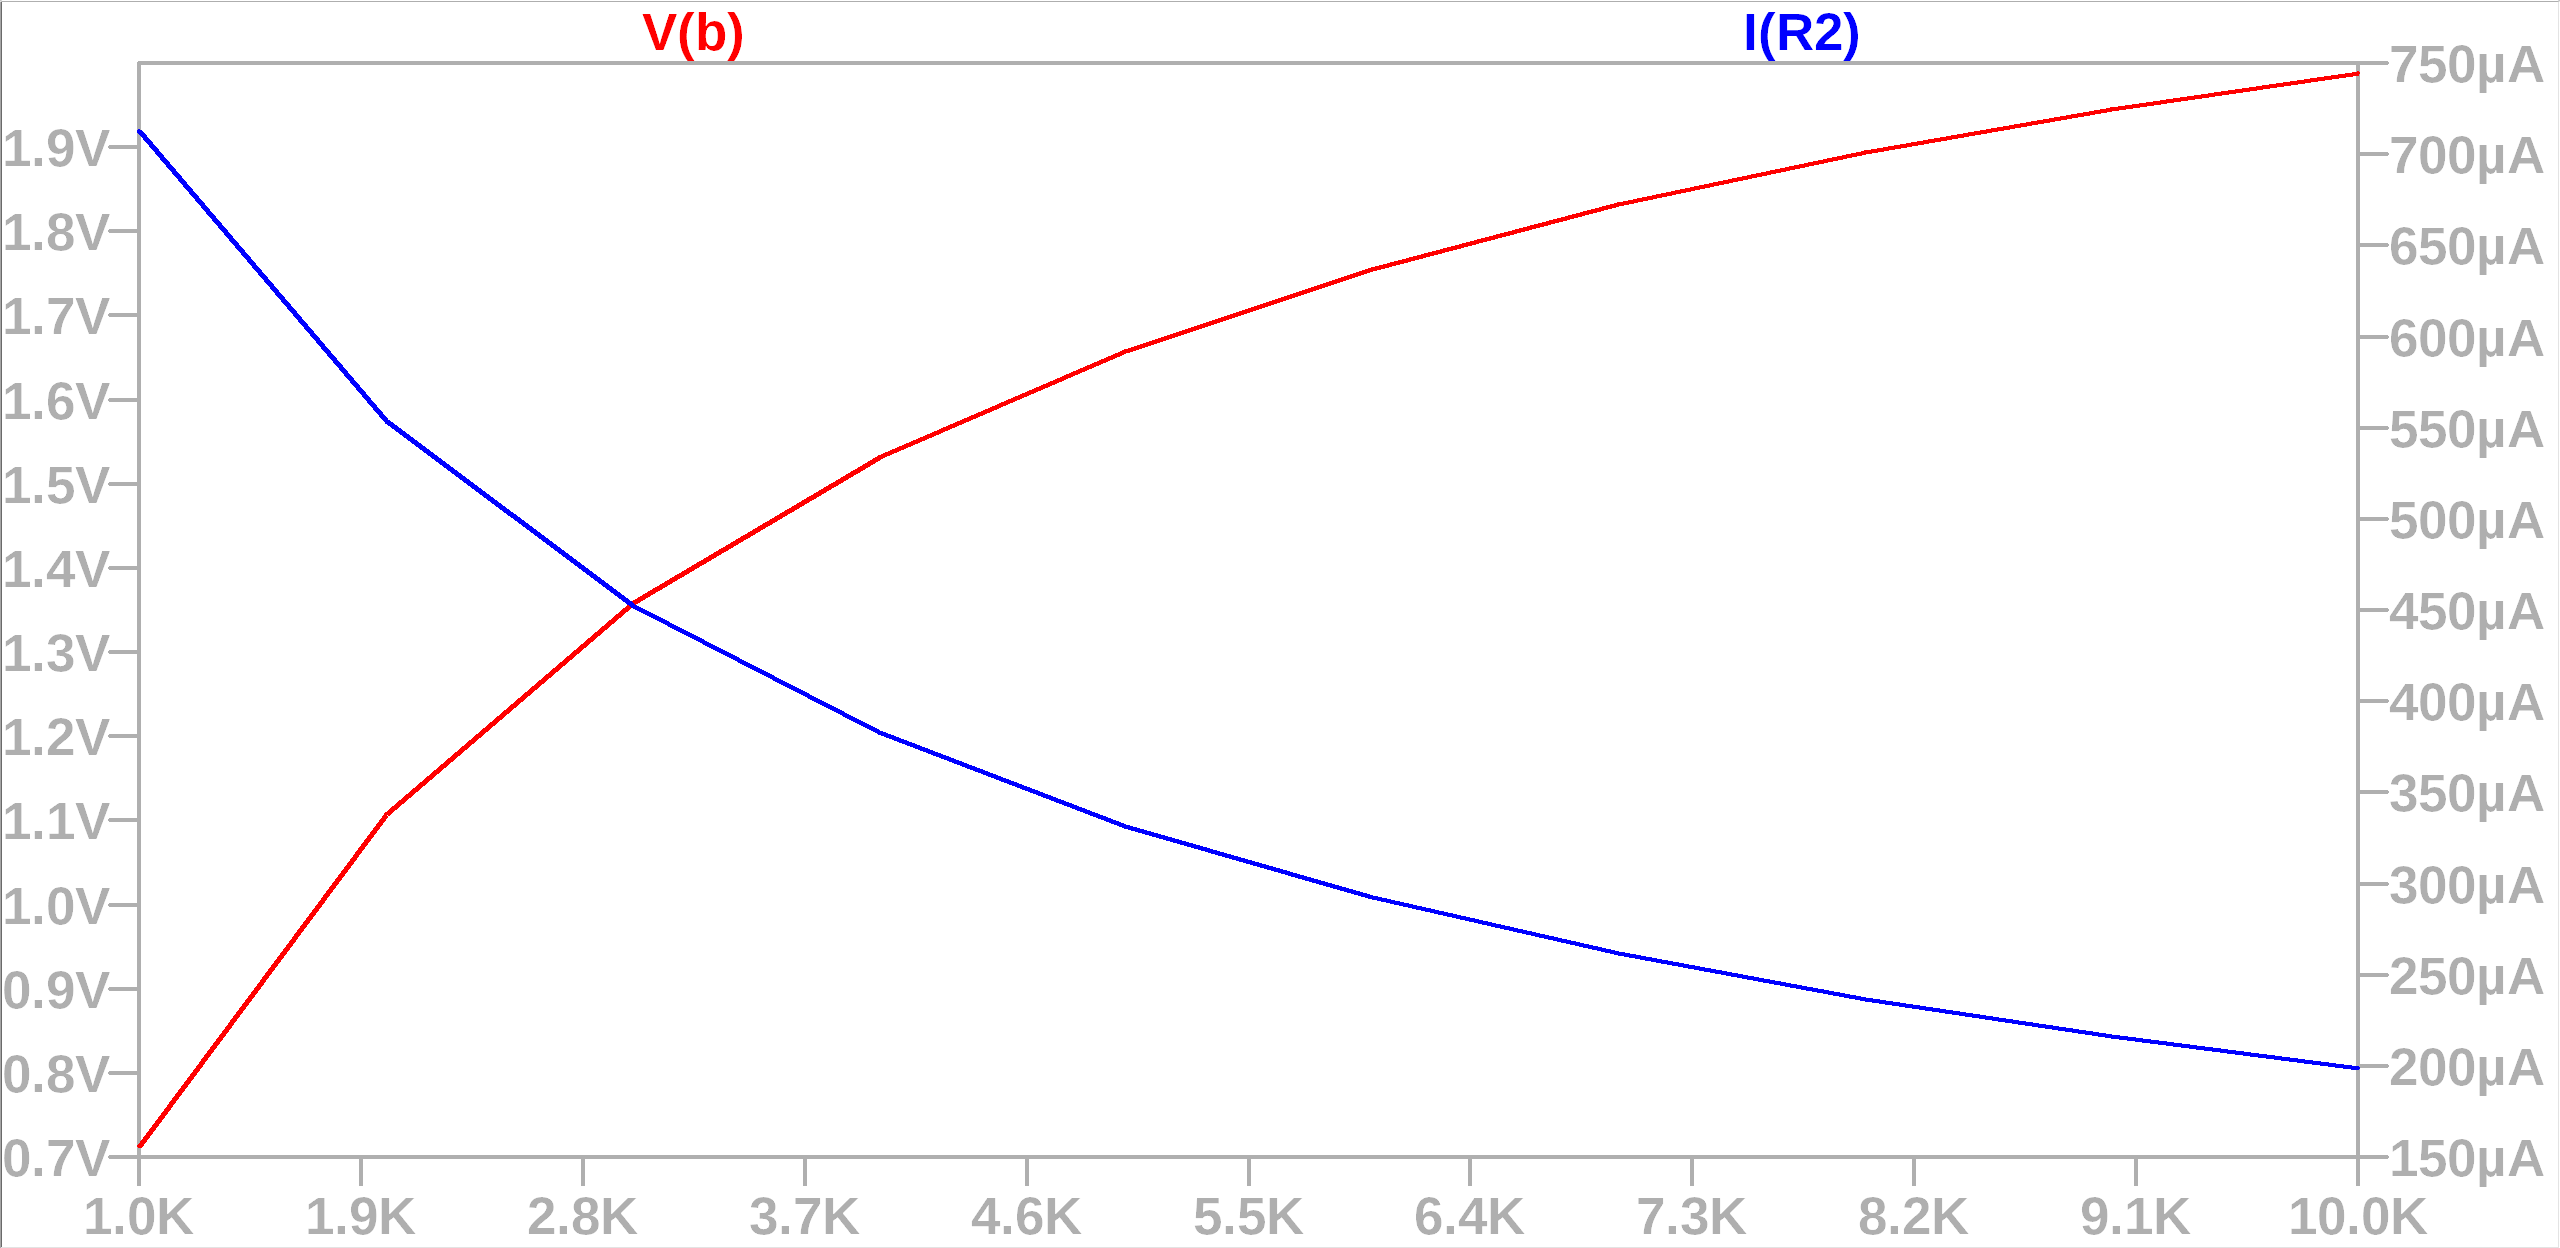
\includegraphics[width=1\textwidth]{image/ltspice_paramsweep_curvas.png}
    \caption{Tensión y corriente en $R_2$ vs valor de $R_2$.}
\end{figure}
 
% ══════════════════════════════════════════════════════════════════════════════
\section{Implementación y Mediciones}
 
\subsection{Medición de resistores}
 
Previo al armado del circuito, se midieron los resistores con el multímetro
para verificar que sus valores se encuentren dentro de la tolerancia nominal.
 
\begin{table}[H]
\centering
\caption{Tabla 4 --- Valores nominales y medidos de los resistores}
\renewcommand{\arraystretch}{1.5}
\begin{tabular}{lccc}
\toprule
Valor   & $R_1$ & $R_2$ & $R_3$ \\
\midrule
Nominal & $10\,\text{k}\Omega$ & $4{,}7\,\text{k}\Omega$ & $3{,}3\,\text{k}\Omega$ \\
Medido  & $9,96\,\text{k}\Omega$ & $4,73\,\text{k}\Omega$ & $3,302\,\text{k}\Omega$ \\
\bottomrule
\end{tabular}
\end{table}
 
\subsection{Armado del circuito en protoboard}
 
\begin{figure}[H]
    \centering
    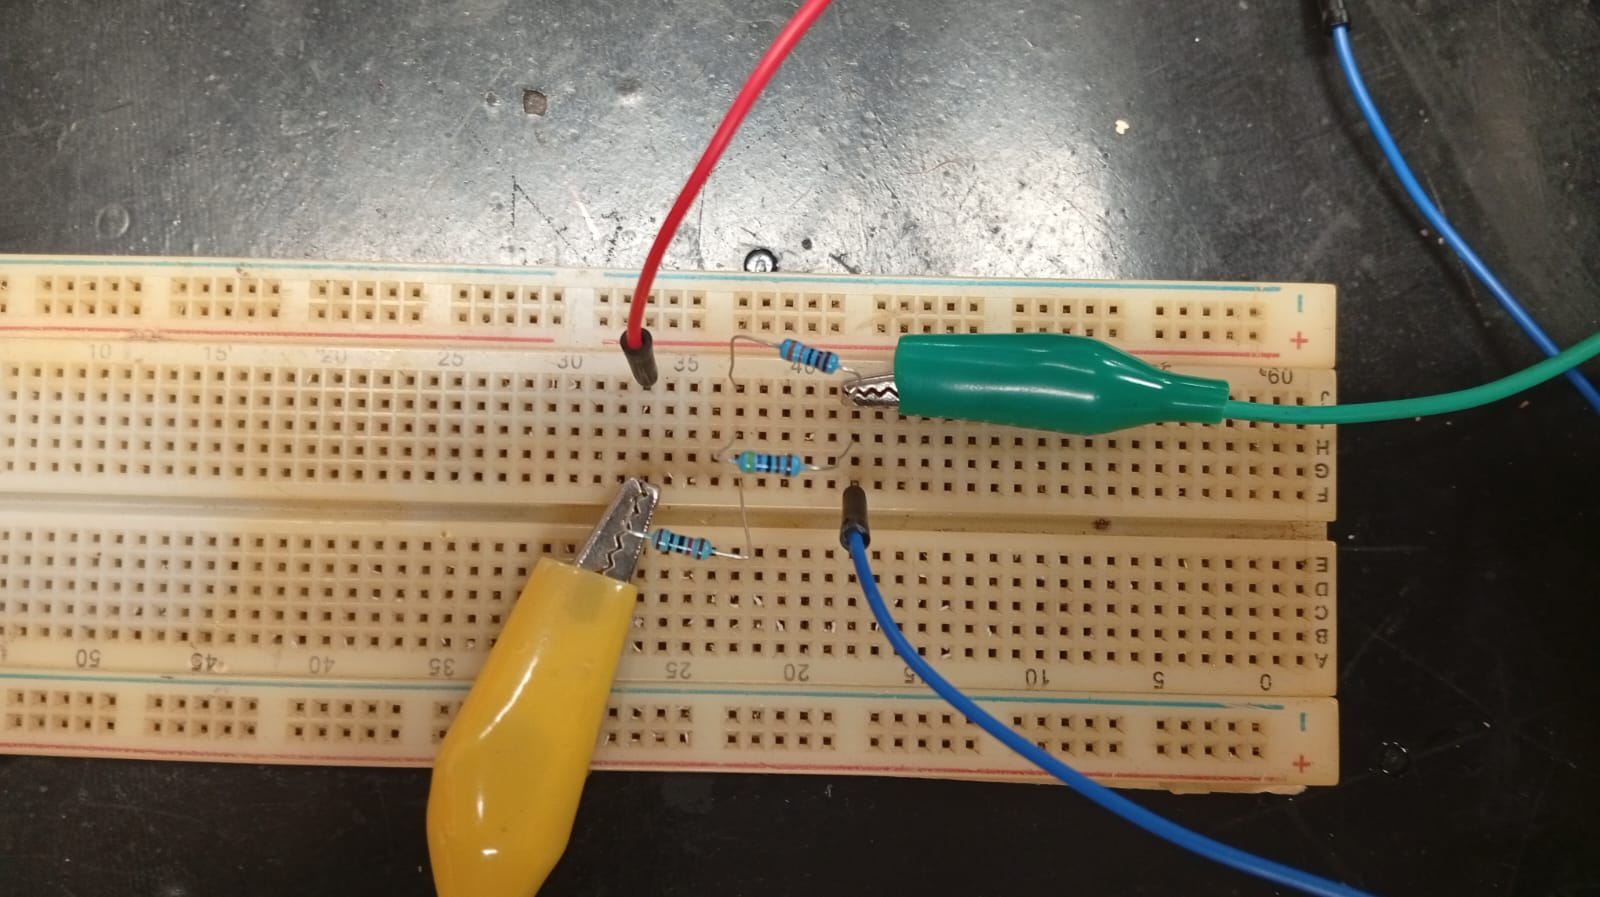
\includegraphics[width=0.75\textwidth]{image/Protoboard.jpeg}
    \caption{Circuito implementado en protoboard con $V_S = 10\,\text{V}$.}
\end{figure}
 
\subsection{Mediciones de tensiones}
 
\begin{figure}[H]
    \centering
    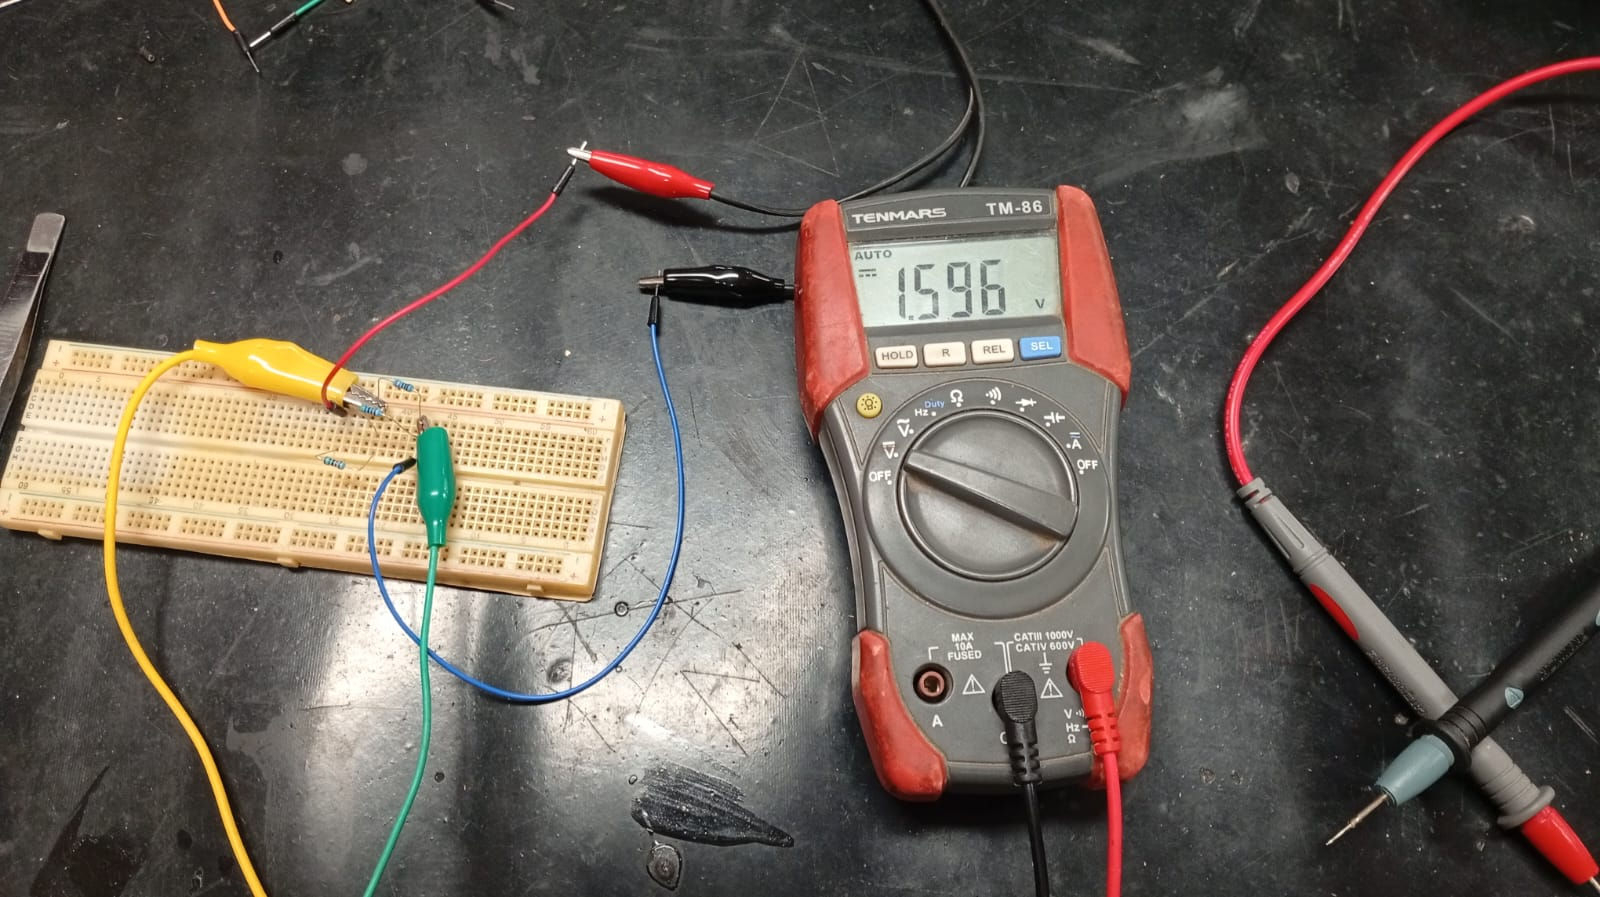
\includegraphics[width=0.75\textwidth]{image/Multimetro.jpeg}
    \caption{Medición de tensiones con multímetro sobre el circuito implementado.}
\end{figure}
 
\subsection{Tabla de valores medidos}
 
\begin{table}[H]
\centering
\caption{Tabla 5 --- Valores medidos en la implementación}
\renewcommand{\arraystretch}{1.5}
\begin{tabular}{lcccc}
\toprule
 & $V_S$ & $R_1$ & $R_2$ & $R_3$ \\
\midrule
Tensión   & 10V & 8,24V & 1,602V & 1,602V \\
 Corriente   & $831\,\mu\text{A}$ & $837\,\mu\text{A}$ & $327\,\mu\text{A}$ & $482\,\mu\text{A}$ \\
 Potencia    & $8{,}31\,\text{mW}$ & $6{,}89\,\text{mW}$ & $0{,}523\,\text{mW}$ & $0{,}772\,\text{mW}$ \\
\bottomrule
\end{tabular}
\end{table}
 
\subsection{Comparación Análisis --- Simulación --- Medición}
 
\begin{table}[H]
\centering
\caption{Tabla 6 --- Comparación de resultados obtenidos por los tres métodos}
\renewcommand{\arraystretch}{1.5}
\begin{tabular}{llcccc}
\toprule
 & Método & $V_S$ & $R_1$ & $R_2$ & $R_3$ \\
\midrule
\multirow{3}{*}{Tensión}
    & Análisis   & 10V & 8,376V & 1,623V & 1,623V \\
    & Simulación & 10V & 8,376V & 1,624V & 1,624V \\
    & Medición   & 10V & 8,24V & 1,602V & 1,602V \\
\midrule
\multirow{3}{*}{Corriente}
    & Análisis    &  $837{,}6\,\mu\text{A}$ & $837{,}6\,\mu\text{A}$ & $345{,}5\,\mu\text{A}$ & $492{,}1\,\mu\text{A}$ \\
    & Simulación & $838{,}0\,\mu\text{A}$ & $838{,}0\,\mu\text{A}$ & $345{,}6\,\mu\text{A}$ & $492{,}1\,\mu\text{A}$ \\
    & Medición   & $831\,\mu\text{A}$ & $837\,\mu\text{A}$ & $327\,\mu\text{A}$ & $482\,\mu\text{A}$ \\
\midrule
\multirow{3}{*}{Potencia}
    & Análisis   &  $8{,}376\,\text{mW}$ & $7{,}016\,\text{mW}$  & $0{,}561\,\text{mW}$ & $0{,}799\,\text{mW}$ \\
    & Simulación & $8{,}376\,\text{mW}$ & $7{,}016\,\text{mW}$ & $0{,}561\,\text{mW}$ & $0{,}799\,\text{mW}$ \\
    & Medición   & $8{,}31\,\text{mW}$ & $6{,}89\,\text{mW}$ & $0{,}523\,\text{mW}$ & $0{,}772\,\text{mW}$ \\
\bottomrule
\end{tabular}
\end{table}
 
% ══════════════════════════════════════════════════════════════════════════════
\section{Conclusiones}
 
A continuación se responden las preguntas propuestas por la cátedra
a partir de las actividades realizadas en el TP1.
 
\begin{enumerate}[leftmargin=*, label=\textbf{\arabic*.}]
 
    \item \textbf{Selección de potencia nominal de los resistores.}\\
    Basándose en los cálculos de potencia realizados en la Actividad 2,
    ¿fueron correctamente seleccionadas las potencias nominales
    ($\frac{1}{4}$\,W o $\frac{1}{8}$\,W) de los componentes utilizados?\\[4pt]
    Aunque es cierto que las potencias disipadas por las resistencias en las mediciones prácticas difieren levemente con las potencias calculadas en el análisis, podemos definir que las potencias nominales de las resistencias usadas son correctas, ya que están muy por debajo de la potencia máxima que pueden disipar sin dañarse.
 
    \item \textbf{Porcentaje de disipación y vida útil.}\\
    ¿Qué porcentaje de su capacidad máxima de disipación está operando
    cada resistor y cómo afectaría esto a su vida útil en un diseño permanente?\\[4pt]
    El porcentaje de uso se calcula como $\%P = P_{\text{disipada}} / P_{\text{nominal}} \times 100$. \\
    $$\%P_{R_1} = 6{,}89\,\text{mW} / 125\,\text{mW} \times 100 = 2{,}756\%$$
    $$\%P_{R_2} = 3{,}47\,\text{mW} / 125\,\text{mW} \times 100 = 1{,}388\%$$
    $$\%P_{R_3} = 5{,}12\,\text{mW} / 125\,\text{mW} \times 100 = 2{,}048\%$$
    \\
    Las tres resistencias operan por debajo del 3\% de su capacidad máxima. Este margen es más que adecuado para uso continuo, sin riesgo de degradación térmica ni reducción de vida útil. \\
 
    \item \textbf{Limitaciones del modelo SPICE respecto al entorno real.}\\
    ¿Qué factores del entorno real no contempla la simulación DC op point en LTspice?\\[4pt]
    La simulación asume componentes ideales: resistencias exactamente nominales, fuente de tensión perfecta y conexiones sin resistencia. No contempla la tolerancia de los componentes, la resistencia de contacto en la protoboard, la resistencia interna de la fuente, ni variaciones por temperatura.
 
    \item \textbf{Influencia del Parameter Sweep en la estabilidad de tensiones.}\\
    Tras realizar el barrido en $R_2$, ¿en qué medida su variación afecta
    las tensiones en el resto de los nodos?\\[4pt]
    [Describir el comportamiento observado en las gráficas:
    cómo varía $V_B$, $I_2$, $I_3$ al cambiar $R_2$.]
 
    \item \textbf{Influencia de la tolerancia en los valores medidos.}\\
    ¿Cómo influyó la tolerancia de los resistores reales
    en la desviación de los valores de corriente medidos respecto a los teóricos?\\[4pt]
    La mayor desviación se da en $R2$, consistente con que los resistencias comerciales de 5\% de tolerancia (banda dorada)
    pueden alejarse hasta ese porcentaje del valor nominal. Las diferencias observadas se encuentran dentro del rango esperado.
 
    \item \textbf{Resistencia interna del multímetro.}\\
    ¿Es posible que la resistencia interna del multímetro al medir corriente
    haya alterado el comportamiento del circuito original?\\[4pt]
    La resistencia interna de un amperímetro digital es típicamente del orden de un ohm a diez ohm. Frente a las
    resistencias del circuito, que son del orden de los kilo ohm, este valor es despreciable (<0,1\% de la resistencia
    total). Por lo tanto, la inserción del multímetro no alteró significativamente el comportamiento del circuito.
 
    \item \textbf{Método más confiable para toma de decisiones en diseño.}\\
    Si los valores medidos difieren de los simulados, ¿qué método considera
    más confiable y bajo qué argumentos?\\[4pt]
    Los tres métodos son complementarios. El análisis teórico establece el comportamiento ideal y sirve como referencia.
    La simulación permite verificar rápidamente sin montar el circuito, pero depende de la precisión del modelo. La
    medición sobre el prototipo real es la validación definitiva, ya que incorpora todos los efectos del entorno físico.
    La decisión de diseño debe basarse en la medición, usando análisis y simulación como herramientas de predicción y
    detección de errores.
 
    \item \textbf{Variaciones en la tabla comparativa (Tabla 6).}\\
    ¿Se notaron variaciones entre los valores de tensión y corriente
    en los tres entornos (análisis, simulación y medición)?
    ¿Qué factores contribuyen a estas diferencias?\\[4pt]
    Las variaciones entre los tres métodos son pequeñas y explicables. En tensión, la mayor diferencia está en $R2$,
    esto es atribuible a la tolerancia real del componente. En potencia, la medición arroja valores algo distintos a los
    calculados porque parte de diferencias acumuladas en tensión y corriente. Los factores principales son: tolerancia de
    los resistores, resistencia de contacto en la protoboard, y precisión de la escala del multímetro utilizada.
 
\end{enumerate}
 
% ══════════════════════════════════════════════════════════════════════════════
\section{Bibliografía / Referencias}
 
\begin{itemize}
    \item Floyd, Thomas L.\ \textit{Principles of Electric Circuits: Conventional
    Current Version}. Pearson Prentice Hall, 2007.
 
    \item González, Mónica Liliana. \textit{LTSPICE Análisis de circuitos y
    dispositivos electrónicos}, 1\textsuperscript{a} ed.\ La Plata, EDULP, 2018.
    Disponible en: \url{http://sedici.unlp.edu.ar/handle/10915/69818}.
\end{itemize}
 
%--------------------------------
\end{document}